\chapter{Descripción y funcionamiento del producto}\label{ch:description}

\section{Finalidad}
Los cuadros \ReplicaGenOne{} y \ReplicaNextLong{} sustituyen a los conjuntos de instrumentos originales de Volkswagen y amplían su funcionalidad. Ofrecen indicaciones digitales de velocidad, régimen del motor, temperatura del refrigerante, nivel de combustible y cálculos auxiliares de la MFA, y son compatibles tanto con sensores de velocidad por cable como electrónicos. Las unidades \ReplicaGenOneShort{} integran un controlador Bluetooth, mientras que \ReplicaNextShort{} añade módulos de configuración mediante Wi-Fi y unidades de expansión opcionales.

\section{Identificación del modelo}
Cada cuadro está marcado con un código de cuatro letras que describe la cadena cinemática, el tipo de montaje, la interfaz del sensor de velocidad y la generación del mazo. Dígitos opcionales indican la escala admitida del cuentarrevoluciones, y un sufijo adicional de tres letras informa sobre las unidades de medida para exportación.

\subsection{Designación de cuatro letras}
\begin{description}
    \item[Posición~1] \textbf{G} para motores de gasolina o \textbf{D} para motores diésel.
    \item[Posición~2] \textbf{A} para unidades ensambladas en fábrica o \textbf{M} para kits de autoensamblaje.
    \item[Posición~3] \textbf{C} para sensor de velocidad mecánico por cable o \textbf{R} para sensor de velocidad electrónico.
    \item[Posición~4] \textbf{T} para el mazo anterior al facelift (CE~1) o \textbf{S} para el mazo posterior (CE~2).
\end{description}
Un dígito final indica la velocidad máxima mostrada del motor en miles de RPM (por ejemplo, “8” en un cuadro GACT8 equivale a una escala de 8000~RPM).

\subsection{Sufijo de unidades}
Las variantes de exportación pueden añadir un sufijo de tres letras formado a partir del conjunto \texttt{MGFK}:
\begin{description}
    \item[M] millas por hora,
    \item[G] galones,
    \item[F] Fahrenheit,
    \item[K] Kelvin.
\end{description}
Por ejemplo, un cuadro \texttt{GART8-MGF} es una unidad de gasolina, ensamblada en fábrica, con sensor electrónico, mazo CE~2, tacómetro de 8000~RPM y unidades de medida imperiales.

\section{Gama de modelos}
{\scriptsize
\begin{tblr}{
    colspec={Q[l,2.2cm] X[l]},
    hlines
}
\textbf{Modelo} & \textbf{Descripción} \\
GACT & Gasolina, completamente ensamblado, sensor de velocidad por cable, dos conectores, escala de 7000~RPM. \\
GART & Gasolina, completamente ensamblado, sensor de velocidad electrónico remoto, dos conectores, escala de 7000~RPM. \\
GAC & Gasolina, completamente ensamblado, sensor de velocidad por cable, un conector, escala de 7000~RPM. \\
GARS & Gasolina, completamente ensamblado, sensor de velocidad electrónico remoto, un conector, escala de 7000~RPM. \\
GACT8 & Gasolina, completamente ensamblado, sensor de velocidad por cable, dos conectores, escala de 8000~RPM. \\
GART8 & Gasolina, completamente ensamblado, sensor de velocidad electrónico remoto, dos conectores, escala de 8000~RPM. \\
GACS8 & Gasolina, completamente ensamblado, sensor de velocidad por cable, un conector, escala de 8000~RPM. \\
GARS8 & Gasolina, completamente ensamblado, sensor de velocidad electrónico remoto, un conector, escala de 8000~RPM. \\
DACT & Diésel, completamente ensamblado, sensor de velocidad por cable, dos conectores, escala de 6000~RPM. \\
DART & Diésel, completamente ensamblado, sensor de velocidad electrónico remoto, dos conectores, escala de 6000~RPM. \\
DACS & Diésel, completamente ensamblado, sensor de velocidad por cable, un conector, escala de 6000~RPM. \\
DARS & Diésel, completamente ensamblado, sensor de velocidad electrónico remoto, un conector, escala de 6000~RPM. \\
MT & Kit de autoensamblaje con dos conectores. \\
M.S. & Kit de autoensamblaje con un conector. \\
NEXT-GART & \ReplicaNextLong{}, escala de 8000~RPM, dos conectores, sensor de velocidad electrónico. \\
NEXT-GARS & \ReplicaNextLong{}, escala de 8000~RPM, un conector, sensor de velocidad electrónico. \\
NEXT-MT & Kit de autoensamblaje \ReplicaNextLong{} con dos conectores. \\
NEXT-MS & Kit de autoensamblaje \ReplicaNextLong{} con un conector. \\
\end{tblr}}

\section{Asignación de pines de los conectores}
\subsection{Cuadros con dos conectores}
\begin{figure}[htbp]
    \centering
    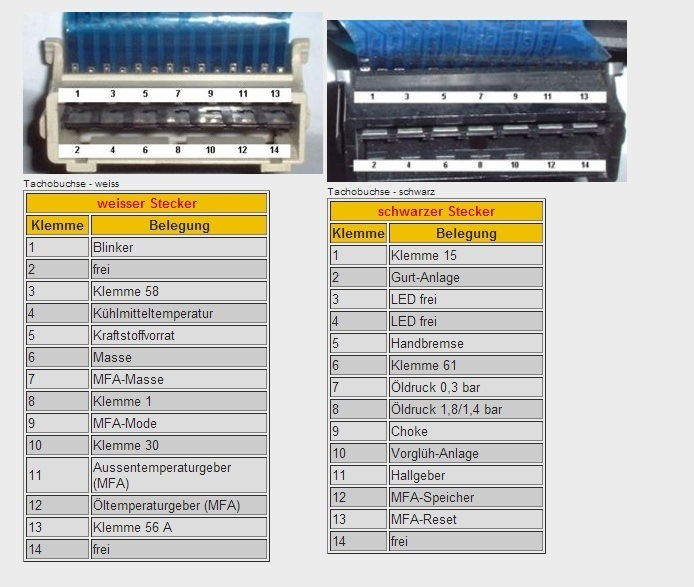
\includegraphics[width=0.72\textwidth]{digifiz_manual/image008.jpg}
    \caption{Distribución de conectores para cuadros \ReplicaGenOne{} con dos enchufes.}
\end{figure}

\noindent\textbf{Conector blanco}

{\scriptsize
\begin{tblr}{
    colspec={Q[l,1.4cm] X[l]},
    hlines
}
\textbf{Pin} & \textbf{Asignación} \\
1 & Salida de intermitente, conectada a masa para la lámpara indicadora. \\
2 & Frei — sin conexión. \\
3 & Terminal~58, alimentación positiva para la retroiluminación del panel. \\
4 & Entrada del sensor resistivo de temperatura del refrigerante. \\
5 & Entrada del sensor resistivo del nivel de combustible. \\
6 & Retorno de masa. \\
7 & Retorno de masa adicional. \\
8 & Señal de régimen del motor en el terminal~1 (bobina, distribuidor u otra forma de onda de hasta 12~V con posibles picos de 300~V). \\
9 & Línea de modo MFA utilizada para cambiar las funciones de la MFA. \\
10 & Alimentación positiva permanente UNR (sin uso en \ReplicaGenOneShort{}, alimentación principal en \ReplicaNextShort{}). \\
11 & Conductor “+” de temperatura MFA para el sensor ambiental (\ReplicaNextShort{}). \\
12 & Conductor del sensor de temperatura de aceite MFA (solo \ReplicaNextShort{}). \\
13 & Entrada del indicador de luces largas KL~56a (+12~V activo). \\
\end{tblr}}

\noindent\textbf{Conector negro}

{\scriptsize
\begin{tblr}{
    colspec={Q[l,1.4cm] X[l]},
    hlines
}
\textbf{Pin} & \textbf{Asignación} \\
1 & Terminal~15, +12~V conmutados desde el interruptor de encendido. \\
2--4 & Sin conexión. \\
5 & Entrada del indicador de freno de mano (activo en bajo). \\
6 & Salida de la lámpara de advertencia del generador KL~61 con resistencia de excitación de 120~\ensuremath{\Omega}. \\
7 & Interruptor de presión de aceite, 0.3~bar. \\
8 & Interruptor de presión de aceite, 1.8~bar. \\
9 & Sin uso. \\
10 & Entrada del indicador de precalentamiento (+12~V activo, solo diésel). \\
11 & Entrada de sensor Hall para sensores de velocidad opcionales. \\
12 & Línea de selección de bloque MFA. \\
13 & Línea de reinicio MFA. \\
\end{tblr}}

\subsection{Cuadros con un solo conector}
Los cuadros con un único conector utilizan la asignación mostrada en \autoref{fig:single-connector}. El mazo reproduce las mismas señales presentes en las variantes de dos conectores, pero las concentra en un único enchufe.

\begin{figure}[htbp]
    \centering
    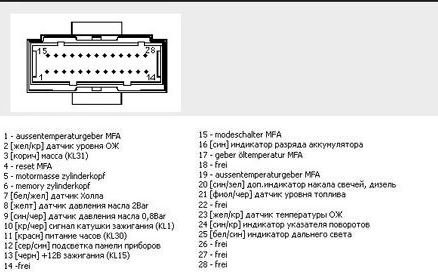
\includegraphics[width=0.65\textwidth]{digifiz_manual/image009.png}
    \caption{Distribución de un solo conector utilizada en los cuadros Replica compactos.}
    \label{fig:single-connector}
\end{figure}

\subsection{Mazo prospectivo Scirocco/Passat}
El mazo prospectivo para Scirocco/Passat utiliza dos conectores. Sus funciones se resumen a continuación.

\noindent\textbf{Conector de 5 pines}
{\scriptsize
\begin{tblr}{
    colspec={Q[l,2.6cm] X[l]},
    hlines
}
\textbf{Pin} & \textbf{Asignación} \\
1~(D3) & Contacto del indicador de la gama “D” de la transmisión automática. Conecta a masa la lámpara de marcha cuando el selector está en posición~D. \\
2~(D2) & Contacto del indicador de la segunda gama de la transmisión automática. Conecta a masa la lámpara “2” cuando el selector está en posición~2. \\
3~(D1) & Contacto del indicador de la gama baja de la transmisión automática. Conecta a masa la lámpara “1” cuando el selector está en posición~1. \\
4~(SA) & Alimentación común para la indicación del selector automático (\emph{Schaltanzeige}); proporciona los +12~V para las lámparas de gama. \\
5~(SPERRE) & Contacto del bloqueo de arranque proveniente del selector. Cerrado en estacionamiento o punto muerto para permitir el arranque del motor. \\
\end{tblr}}

\noindent\textbf{Conector de 14 pines}
{\scriptsize
\begin{tblr}{
    colspec={Q[l,2.6cm] X[l]},
    hlines
}
\textbf{Pin} & \textbf{Asignación} \\
1~(KL~58) & Alimentación de iluminación para la retroiluminación del panel. \\
2~(MASS) & Retorno de masa del chasis. \\
3~(TANK) & Entrada del aforador de combustible. \\
4~(TEMP) & Entrada del sensor de temperatura del refrigerante. \\
5~(KL~1) & Señal de régimen del motor (terminal~1). \\
6~(UHR) & +12~V permanente para el reloj y la memoria. \\
7~(FERNL) & Entrada del indicador de luces largas. \\
8~(reserved) & Sin conexión. \\
9~(OEL~1.8) & Interruptor de alta presión de aceite, 1.8~bar. \\
10~(CAT~VORGL(-)) & Entrada de la lámpara de precalentamiento catalítico / precalentamiento diésel (activa en bajo). \\
11~(OEL~0.3) & Interruptor de baja presión de aceite, 0.3~bar. \\
12~(KL~61) & Lámpara de advertencia del alternador y alimentación de excitación. \\
13~(KL~49a) & Alimentación combinada del indicador de intermitentes. \\
14~(KL~15) & Alimentación +12~V conmutada por el encendido. \\
\end{tblr}}

\subsection{Asignación de conectores para Mk1}
Los vehículos Volkswagen Mk1 utilizan las siguientes asignaciones:
\begin{enumerate}
    \item Alimentación de iluminación y luces de cruce.
    \item Referencia de masa MASSE~31.
    \item Aforador de combustible TANK.
    \item Sensor de temperatura TEMP.
    \item Señal de cuentarrevoluciones KL~1.
    \item +12~V permanente UHR.
    \item Señal de luces largas KL~56.
    \item Interruptor de presión de aceite (ALTA) 1.8~bar.
    \item Interruptor de presión de aceite (BAJA) 0.3~bar.
    \item Indicador de precalentamiento diésel.
    \item Entrada CHOKE (sin uso).
    \item Lámpara del generador KL~61.
    \item Entrada del intermitente (combinado izquierda/derecha).
    \item Alimentación de encendido KL~15.
\end{enumerate}
\begin{figure}[htbp]
    \centering
    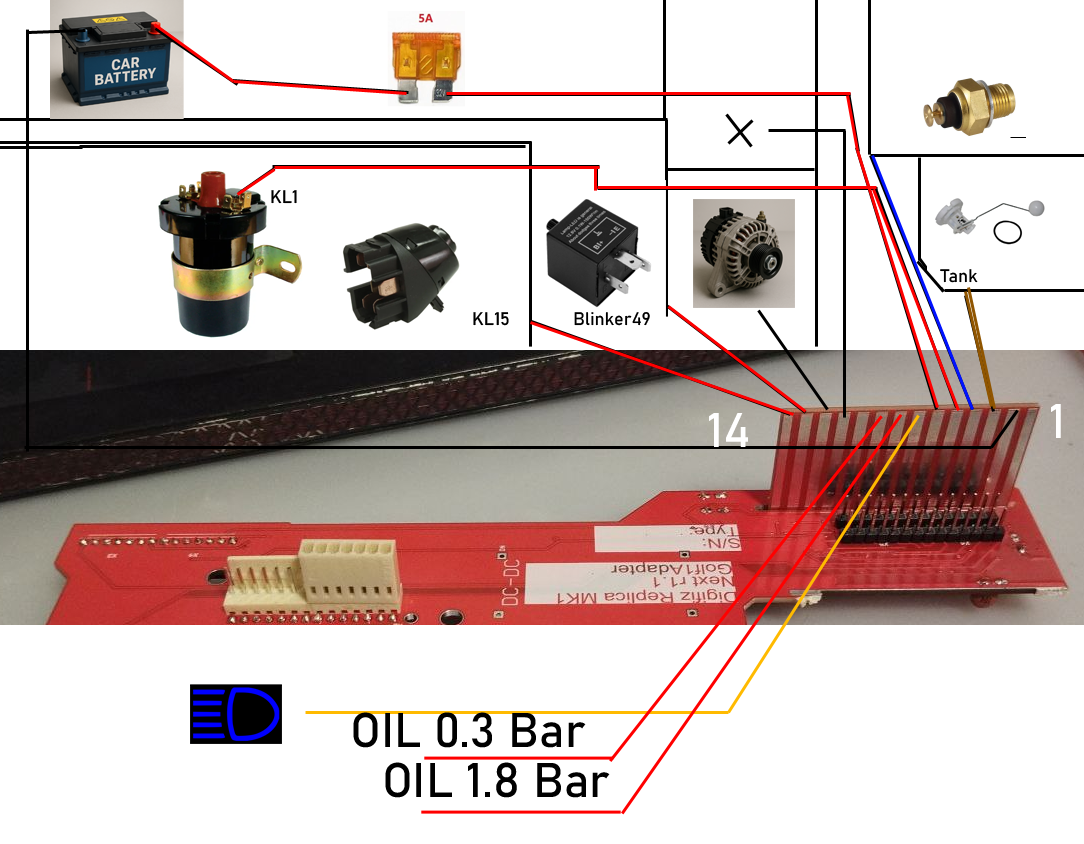
\includegraphics[width=0.75\textwidth]{digifiz_manual/image010.png}
    \caption{Diagrama de conexión del mazo para instalaciones Mk1.}
\end{figure}

\subsection{Conector de servicio de la placa de circuito impreso}
El tercer conector de la placa replica los conectores del cuadro, con pines numerados de derecha a izquierda en las unidades \ReplicaGenOneShort{} y \ReplicaNextShort{}. Proporciona una interfaz de servicio con las asignaciones listadas en \autoref{tab:service-connector}.

\begin{table}[htbp]
    \centering
    \caption{Asignaciones del conector de servicio.}
    \label{tab:service-connector}
    {\scriptsize
    \begin{tblr}{
        colspec={Q[l,1.9cm] X[l]},
        hlines,
    }
        \textbf{Posición} & \textbf{Asignación} \\
        1 & Salida de indicador. \\
        2 & Entrada del sensor de velocidad (SPM\_M). \\
        3 & Masa del vehículo. \\
        4 & Salida de indicador. \\
        5 & Entrada del optoacoplador del intermitente izquierdo. \\
        6 & Entrada del optoacoplador del intermitente derecho. \\
        7 & +12~V de encendido. \\
        8 & Entrada específica para diésel. \\
        9 & Entrada de indicador (positiva). \\
        10 & Entrada alternativa de RPM (sin uso, solo \ReplicaNextShort{}). \\
        11 & \ReplicaGenOneShort{}: salida de indicador (normalmente desconectada); \ReplicaNextShort{}: entrada de freno (activa en bajo). \\
        12 & Reservado. \\
        13 & Entrada de check engine. \\
        14 & Sin contacto. \\
    \end{tblr}}
\end{table}

\subsection{Conectores de expansión auxiliares}
En la placa principal se instalan tres cabeceras adicionales de cuatro pines para simplificar las ampliaciones del mazo y los trabajos de servicio:
\begin{itemize}
    \item \textbf{Señales analógicas de expansión:} proporciona un punto de conexión dedicado para entradas analógicas adicionales al integrar sensores personalizados.
    \item \textbf{Espejo de la MFA:} duplica el conector \textsc{MFA} estándar para admitir la derivación en paralelo de las señales del ordenador de viaje.
    \item \textbf{Duplicados analógicos:} repite las entradas de temperatura de aceite, temperatura ambiente e indicador de freno para que estos circuitos puedan rutearse a módulos externos de registro o monitorización.
\end{itemize}
Los tres utilizan el conector \mbox{KF2510-4p}, que no se suministra con el kit del cuadro y debe adquirirse por separado en caso necesario.

\begin{figure}[htbp]
    \centering
    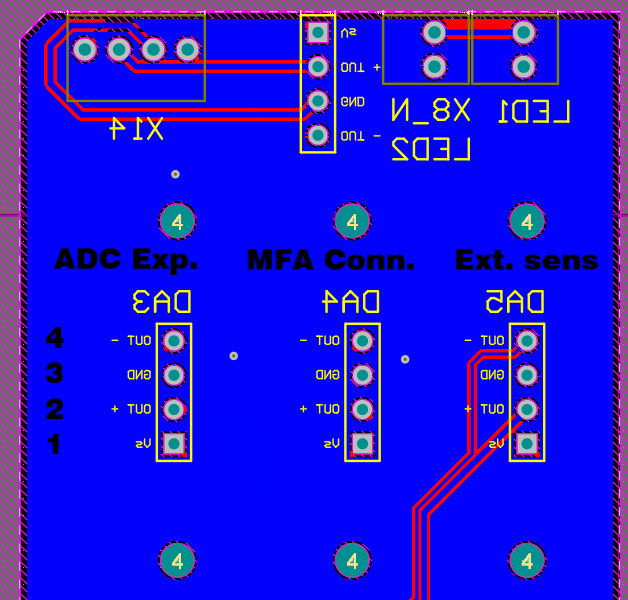
\includegraphics[width=0.6\textwidth]{digifiz_manual/ext_conn.png}
    \caption{Distribución de los conectores auxiliares en la placa principal.}
\end{figure}

\begin{table}[htbp]
    \centering
    {\small
    \begin{tblr}{
        colspec={Q[l,2.3cm] Q[c,1.3cm] X[l]},
        hlines,
        row{1} = {font=\bfseries}
    }
    Conector & Pin & Asignación \\
    Conector~I & 4 & Entrada analógica auxiliar~1 \\
    Conector~I & 3 & Masa (GND) \\
    Conector~I & 2 & Entrada analógica auxiliar~2 \\
    Conector~I & 1 & VCC (3V3, sin fusible\textbf{!!!}) \\
    Conector~II & 4 & Reinicio MFA \\
    Conector~II & 3 & Masa (GND) \\
    Conector~II & 2 & Bloque de memoria MFA \\
    Conector~II & 1 & Modo MFA \\
    Conector~III & 4 & Salida del sensor de temperatura de aceite \\
    Conector~III & 3 & Masa (GND) \\
    Conector~III & 2 & Salida del sensor de temperatura exterior \\
    Conector~III & 1 & Indicador de freno \\
    \end{tblr}}
    \caption{Asignaciones de los conectores de expansión auxiliares.}
\end{table}

\section{Software integrado y contenido del suministro}
El firmware del cuadro se publica en la siguiente dirección:
\displayurl{https://github.com/Sgw32/DigifizReplica}
Hay dos juegos de entrega disponibles:
\begin{itemize}
    \item \textbf{\ReplicaGenOne{}:} conjunto del cuadro, mazo de temperaturas ambiente y de aceite, programador USBasp y, para sensores remotos, mazo del sensor de velocidad.
    \item \textbf{\ReplicaNextLong{}:} conjunto del cuadro y mazo del sensor de velocidad electrónico.
\end{itemize}
